\section{Problem Formulation from Global Perspective}
%----------------------------------------------------------------------------------------%
In this section, we formulate the optimization problem which aims at online joint optimizing job dispatching decisions of all APs.
This kind of optimization problem falls into multi-agent planning problem, which considers a fully cooperative multi-agent system (MAS) and each agent shares the same utility function \needref{Craig Boutilie, 1999}.
In an extensive edge computing network, the transmission latency of information is not negligible and the system state information is always stale due to periodic broadcast and \brlatency.
The stale system state observation is characterized as \emph{partial-observed information} in a branch of MDP problem called Decentralized Partially-Observed MDP (DEC-POMDP).
In \needref{R.Nair, 2003}, the author describes a general multi-agent coordination problem using DEC-POMDP framework. The solution to its problem is of high complexity and requires extra information of \emph{belief states}.

Hence, we formulate our problem from global perspective where the latency of information sharing still exists, but the individual information is assumed available to a centralized agent.
The centralized agent will determine the new policy of each AP based on GSI aware of the \brlatency, and then apply the new policy for each AP at the corresponding \brlatency~time slot in the broadcast interval.
We could obtain optimal solution via Bellman's equation with the MDP problem formulation, and  a low-complexity solution is introduced to alleviate the curse of dimensionality.
And in the next section, we will leverage the problem structure and propose the practical algorithm without centralized agent assumption.

\delete{v7}{Reference list
    [1] "Sequential Optimality and Coordination in Multi-agent Systems", Craig Boutilie, 1999
    [2] "Taming Decentralized POMDPs: Towards Efficient Policy Computation for Multi-agent Settings", R.Nair, 2003
}

\subsection{System State and Dispatching Policy}
We formulate the multi-agent MDP problem from a global perspective, where each AP adopts the dispatching policy mapping from the global broadcast information $\Obsv^{\dagger}$.

\begin{definition}[System State]
    The system state for the $t$-th broadcast interval is denoted as follows.
    \begin{align}
        \Stat(t) \define \Obsv^{\dagger}(t),
    \end{align}
    where $\Obsv^{\dagger}(t)$ is consisted of uploading jobs information and previous dispatching decisions of all APs, and queueing job information of all edge servers at the $t$-th broadcast time slot.
\end{definition}

% the system evolves with the joint actions of all APs.
And the joint policy of all APs is defined as follows.
\begin{definition}[Joint Dispatching Policy]
    The joint dispatching policy $\Policy(\Stat(t))$ over system state $\Stat(t)$ is defined as follows.
    \begin{align}
        \Policy^{\dagger}(\Stat(t)) \define \Brace{
            \Omega^{\dagger}_{1}(\Stat(t)), \dots, \Omega^{\dagger}_{K}(\Stat(t))
        },
    \end{align}
    where $\Omega^{\dagger}_{k}(\Stat(t)) \equiv \Omega^{\dagger}_{k}(\Obsv^{\dagger}(t))$
    is the individual policy of the $k$-th AP ($\forall k\in\apSet$).
\end{definition}
%----------------------------------------------------------------------------------------%

\subsection{The Optimization Problem}
In the edge computing system, each AP individually performs job dispatching decision, and coordinates in a fully cooperative manner by sharing the same utility function.
We propose the job dispatching optimization problem with the target to minimize \emph{average response time} of all offloaded jobs in MEC system.
The \emph{average response time} is composed of uploading time, waiting time and processing time on edge server.
According to \emph{Little's Law}, to minimize the average response time of all jobs is equal to minimize the average number of jobs in the system.

Due to the periodic information broadcasting, we collect the cost for counting numbers each interval, which could be seen as a uniform sampling at times slot scale.
Besides the cost for job response time, we further add penalty on job discarded when the queue is full.
The definition of the cost function is given as follows.
\begin{align}
    g^{\dagger}\Paren{\Stat(t), \Policy^{\dagger}(\Stat(t))} \define
        &\sum_{k\in\apSet} \sum_{m\in\esSet} \sum_{j\in\jSpace} \vec{R}^{(k)}_{m,j}(t)~+
        \nonumber\\
        &\sum_{m\in\esSet} \sum_{j\in\jSpace} \Brace{Q_{m,j}(t) + \beta \cdot \mat{I}[Q_{m,j}(t)=L_{max}]},
\end{align}
where $\beta$ is the weight factor for discard penalty ($\beta \in (0,1)$).

Hence, the online job dispatching problem from global perspective is given as follows.
\begin{problem}[Centralized Job Dispatching Problem]
    \begin{align}
        \min_{\Policy^{\dagger}} \lim_{T \to \infty}
            \mathbb{E}_{\Policy^{\dagger}}
                \Bracket{\sum_{t=1}^t \gamma^{(t-1)} g^{\dagger}\Paren{\Stat(t), \Policy^{\dagger}(\Stat(t))}|\Stat(1)},
    \end{align}
    where the cost is collected with discount factor $\gamma$.
\end{problem}
According to \cite{sutton1998introduction}, the above problem could be solved by the following \emph{Bellman's equation}:
\begin{align}
    V^{\dagger}\Paren{\Stat(t)} =~&g^{\dagger}\Paren{\Stat(t)} + \gamma \min_{\Policy(\Stat(t))}
        \nonumber\\
        &\sum_{\Stat(t+1)} \Pr\Brace{ \Stat(t+1)|\Stat(t), \Policy(\Stat(t)) } \cdot V^{\dagger}\Paren{\Stat(t+1)}.
    \label{eqn:sp_0}
\end{align}

Generally speaking, the optimal policy could be obtained by solving the minimization problem on the right-hand-side of the above Bellman's equation Eqn. (\ref{eqn:sp_0}).
In our problem, however, the conventional value iteration algorithm is intractable due to the tremendous state space.
The number of system states and action space would grow exponentially with respect to the number of APs and edge servers.
Hence, a low-complexity sub-optimal solution is proposed in the next section whose performance is analytically bounded.
\comments{
    Moreover, we remove the assumption on centralized agent by using partial information observed from each AP.
    Then we leverage the low-complexity solution to the global optimization problem and come up with decentralized algorithm.
}

%----------------------------------------------------------------------------------------%
\delete{v7}{
    \begin{figure}[htp]
        \centering
        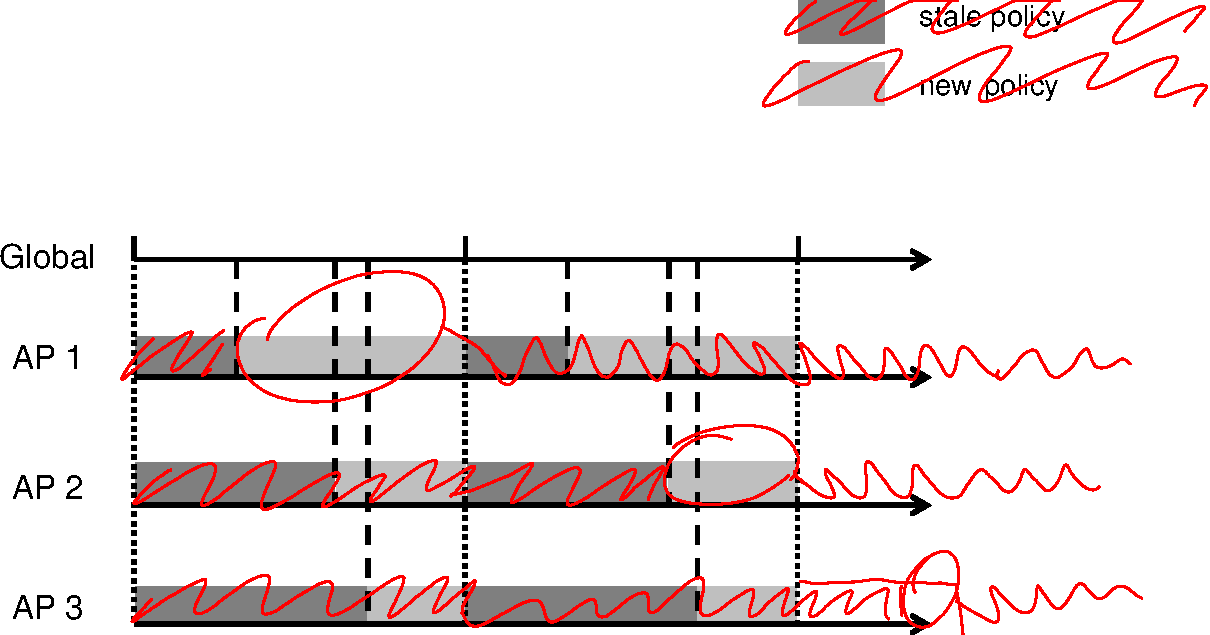
\includegraphics[width=0.80\textwidth]{brd-trans.pdf}
        \caption{Global System Transition with Partial Information-based Dispatching Decision}
        \label{fig:brd-trans}
    \end{figure}
}
%----------------------------------------------------------------------------------------%
